% Created 2014-07-19 Sat 12:40
\documentclass[11pt]{article}
\usepackage[utf8]{inputenc}
\usepackage[T1]{fontenc}
\usepackage{fixltx2e}
\usepackage{graphicx}
\usepackage{longtable}
\usepackage{float}
\usepackage{wrapfig}
\usepackage{rotating}
\usepackage[normalem]{ulem}
\usepackage{amsmath}
\usepackage{textcomp}
\usepackage{marvosym}
\usepackage{wasysym}
\usepackage{amssymb}
\usepackage{hyperref}
\tolerance=1000
\usepackage{listings}
\usepackage{multicol}
\usepackage{enumitem}
\setlist[description]{style=nextline}
\usepackage[compact]{titlesec}
\usepackage[landscape,margin=1cm]{geometry}
\titleformat{\section}[frame]
{\normalfont\sffamily}
{\thesection}{.1em}{\small\bfseries\filcenter}
\titleformat{\subsection}[block]
{\normalfont\sffamily}
{\thesection}{0em}{\scriptsize\bfseries\filcenter}
\titleformat{\subsubsection}[block]
{\normalfont\sffamily}
{\thesection}{0em}{\tiny\bfseries}
\pagestyle{empty}
\makeatletter
\renewcommand{\@maketitle}{
\newpage
\begin{center}%
{\Large\bfseries \@title \par}%
\end{center}%
\par}
\makeatother
\setcounter{secnumdepth}{0}
\setlength{\parindent}{0pt}
\setlength{\parskip}{0pt plus 0.5ex}
\lstset{%
basicstyle=\ttfamily\tiny,
commentstyle=\itshape\ttfamily\tiny,
showspaces=false,
showstringspaces=false,
breaklines=true,
breakautoindent=true,
}
\setlist{wide=0pt,nosep}
\usepackage[default,osfigures]{opensans}
\usepackage[scaled=0.8]{luximono}
\usepackage{hyperref}
\usepackage{amssymb}
\date{}
\title{Yags cheatsheet}
\hypersetup{
 pdfkeywords={},
  pdfsubject={},
  pdfcreator={Emacs 24.3.1 (Org mode 8.3beta)}}
\begin{document}

\maketitle
\begin{multicols}{3}
\scriptsize
\thispagestyle{empty}

\section{Graph definitions}
\label{sec-1}

\begin{description}
\item[{Adjacency list}] \verb~g:=GraphByAdjacencies([[],[4],[1,2],[]])~

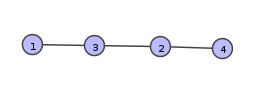
\includegraphics[width=3cm]{bylist.png}
\item[{Adjacency matrix}] \verb~M:=[[false, true, false], [true, false, true], [false, true, false]];~
                      \verb~g:=GraphByAdjMatrix(M);~
\item[{Complete cover}] \verb~g:=GraphByCompleteCover([[1,2,3,4],[4,5,6]]);~

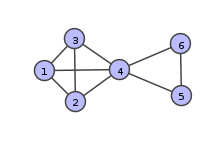
\includegraphics[width=3cm]{bycomplete.png}
\item[{By relation}] \verb~f:=function(x,y) return Intersection(x,y)<>[]; end;;~
                 \verb~g:=GraphByRelation([[1,2,3],[3,4,5],[5,6,7]],f);~
\item[{By walks}] \verb~g:=GraphByWalks([1,2,3,4,1],[1,5,6]);~ 

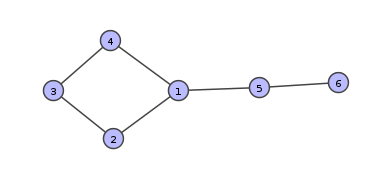
\includegraphics[width=3cm]{bywalks.png}

\verb~g:=GraphByWalks([1,[2,3,4],5],[5,6]);~

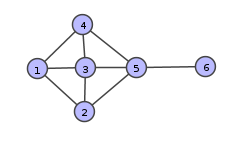
\includegraphics[width=3cm]{bywalks2.png}
\item[{As intersection graph}] \verb~g:=IntersectionGraph([[1,2,3],[3,4,5],[5,6,7]]);~
\item[{As a copy}] \verb~h:=CopyGraph(g)~
\item[{As an induced subgraph}] \verb~h:=InducedSubgraph(g,[3,4,6]);~
\end{description}

\section{Graph families (with parameters)}
\label{sec-2}

\begin{itemize}
\item \verb~g:=DiscreteGraph(n)~
\item \verb~g:=CompleteGraph(n)~
\item \verb~g:=PathGraph(n)~ \(n\) vertices.
\item \verb~g:=CycleGraph(n)~
\item \verb~g:=CubeGraph(n)~
\item \verb~g:=OctahedralGraph(n)~
\item \verb~g:=JohnsonGraph(n,r)~ Vertices are subsets of \(\{1,2,\ldots,n\}\)
with \(r\) elements, edges between subsets with intersection of
\(r-1\) elements.
\item \verb~g:=CompleteBipartiteGraph(n,m)~
\item \verb~g:=CompleteMultipartiteGraph(n1,n2[, n3 ...])~
\item \verb~g:=WheelGraph(n)~
\item \verb~g:=WheelGraph(7,2)~ Second optional parameter is the radius of the
wheel.
\item \verb~g:=FanGraph(4);~
\item \verb~g:=SunGraph(6);~
\item \verb~g:=SpikyGraph(4);~
\item Examples: Wheel, Fan, Sun, Spiky:

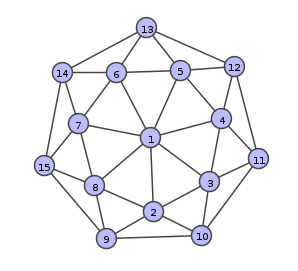
\includegraphics[width=2cm]{wheel.png} 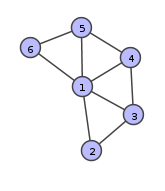
\includegraphics[width=2cm]{fan.png} 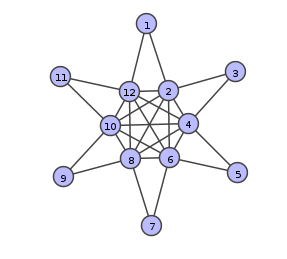
\includegraphics[width=2cm]{sun.png} 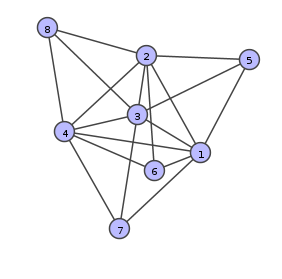
\includegraphics[width=2cm]{spiky.png}
\end{itemize}

\section{Named graphs}
\label{sec-3}
\begin{description}
\item[{Platonic}] \verb~Tetrahedron~, \verb~Octahedron~, \verb~Cube~, \verb~Dodecahedron~, \verb~Icosahedron~.
\item[{Other}] \verb~TrivialGraph~, \verb~DiamondGraph~, \verb~ClawGraph~, \verb~PawGraph~,
\verb~HouseGraph~, \verb~BullGraph~, \verb~AntennaGraph~, \verb~KiteGraph~, \verb~SnubDisphenoid~.
\end{description}
\section{Random graphs}
\label{sec-4}

\begin{itemize}
\item \verb~g:=RandomGraph(n)~
\item \verb~g:=RandomGraph(n,p)~ Graph with \(n\) vertices, each edge with
probability \(p\) to appear.
\end{itemize}

\section{Modifying graphs}
\label{sec-5}

\begin{itemize}
\item \verb~h:=RemoveVertices(g,[1,3]);~
\item \verb~h:=AddEdges(g,[[1,2]]);~
\item \verb~h:=RemoveEdges(g,[[1,2],[3,4]]);~
\end{itemize}

\section{Parameters}
\label{sec-6}

\begin{itemize}
\item \verb~Order(g)~
\item \verb~Size(g)~
\item \verb~CliqueNumber(g)~
\item \verb~VertexDegree(g,v)~
\end{itemize}

\section{Boolean tests}
\label{sec-7}
\begin{itemize}
\item \verb~IsCompleteGraph(g)~
\item \verb~IsCliqueHelly(g)~
\item \verb~IsDiamondFree(g)~
\end{itemize}
\section{Products}
\label{sec-8}
\begin{itemize}
\item \verb~p=BoxProduct(g,h)~
\item \verb~p=TimesProduct(g,h)~
\item \verb~p=BoxTimesProduct(g,h)~
\item \verb~p=DisjointUnion(g,h)~
\item \verb~p=Join(g,h)~
\item \verb~p=GraphSum(g,l)~ \(l\) is a list of graphs. Suppose that \(g\) has
\(n\) vertices. In the disjoint union of the first \(n\) graphs of
\(l\) (using \verb~TrivialGraphs~ if needed to fill \(n\) slots), add all
edges between graphs corresponding to adjacent vertices in \(g\).
\item \verb~p=Composition(g,h)~ is the same as \verb~GraphSum(g,l)~, where \(l\) is
a list of length the order of \(g\), with all components equal to
\(h\).
\end{itemize}

\section{Operators}
\label{sec-9}

\begin{itemize}
\item \verb~h:=CliqueGraph(g)~
\item \verb~h:=CliqueGraph(g,m)~ Stops when a maximum of
\(m\) cliques have been found.
\item \verb~h:=LineGraph(g)~
\item \verb~h:=ComplementGraph(g)~
\item \verb~h:=QuotientGraph(g,p)~ \(p\) is a partition of vertices. The
vertices of \(h\) are the parts of \(p\), with two vertices adjacent
if there are two vertices adjacent in \(g\) in the corresponding
parts. Singletons in \(p\) may be omitted.
\item \verb~h:=QuotientGraph(g,l)~ \(l\) is a pair of lists of vertices of the
same length, with repetitions allowed. In \(h\), each vertex of the
first list is identified with the corresponding vertex in the second
list.
\end{itemize}

\section{Lists}
\label{sec-10}
\begin{itemize}
\item \verb~VertexNames(g)~
\item \verb~Cliques(g)~
\item \verb~Cliques(g,m)~ Stops if a maximum of \(m\) cliques have been found.
\item \verb~AdjMatrix(g)~
\item \verb~Adjaceny(g,v)~
\item \verb~Adjacencies(g)~
\item \verb~VertexDegrees(g)~
\item \verb~Edges(g)~
\item \verb~CompletesOfGivenOrder(g,o)~
\end{itemize}

\section{Distances}
\label{sec-11}
\begin{itemize}
\item \verb~Distance(g,x,y)~
\item \verb~DistanceMatrix(g)~
\item \verb~Diameter(g)~
\item \verb~Eccentricity(g,x)~ 
\item \verb~Radius(g)~
\item \verb~Distances(g,a,b)~ \(a\), \(b\) are lists of vertices. Returns a list.
\item \verb~DistanceSet(g,a,b)~ As before, but returns a set.
\item \verb~DistanceGraph(g,d)~ The graph with vertex set the vertices of
\(g\), two vertices adjacent if their distance is in \(d\).
\item \verb~PowerGraph(g,n)~ Same as the distance graph with set of distance
\(\{1,\ldots,n\}\).
\end{itemize}

\end{multicols}
% Emacs 24.3.1 (Org mode 8.3beta)
\end{document}
